\documentclass[conference]{IEEEtran}
\usepackage{cite}
\usepackage{amsmath,amssymb,amsfonts}
\usepackage{graphicx}
\usepackage{booktabs}
\usepackage{url}

\begin{document}

\title{DWT-DCT Watermark Design Under AI-Based Image Enhancement}

\author{\IEEEauthorblockN{Shiva Tan}
\IEEEauthorblockA{Independent Researcher\\
shivatan21@gmail.com}}

\maketitle

\begin{abstract}
Classical DWT-DCT watermarking is typically evaluated against JPEG
compression, noise, filtering, and geometric attacks. We ask whether
AI-based image enhancement behaves differently. Across 100 images and
four embedding strengths, Real-ESRGAN reduces mean normalized
correlation (NC) from 0.999 to 0.795 while producing the highest
perceptual quality (SSIM 0.885) of any watermark-degrading attack we
evaluated. In contrast, ESPCN, FSRCNN, EDSR, and LapSRN preserve watermark
recovery (NC $\geq 0.999$), showing that the effect is not a property
of learned super-resolution in general, but of GAN-based image
restoration. To understand why, we analyze DCT coefficient changes and
the detector's decision margin. We find that Real-ESRGAN does not
simply perturb embedded coefficients. Instead, it reconstructs local
image content in a signal-dependent way that restores the natural
relationship between DCT coefficients, collapsing the embedded decision
margin and causing bit errors. An exhaustive evaluation of 1,953
coefficient pairs shows that attack-aware coefficient selection
improves robustness to Real-ESRGAN or to JPEG, but not both
simultaneously: the best high-frequency pair raises Real-ESRGAN NC
from 0.783 to 0.831 ($+0.048$, $d=0.89$) while reducing JPEG NC from
0.995 to 0.902. These results suggest that AI-based restoration
represents a fundamentally different attack model for classical
watermarking and that improving robustness will require new embedding
strategies beyond conventional coefficient selection.
\end{abstract}

\begin{IEEEkeywords}
digital watermarking, DWT-DCT, image forensics, robustness evaluation,
super-resolution, AI enhancement, Real-ESRGAN, coefficient selection
\end{IEEEkeywords}

\section{Introduction}
\label{sec:intro}

Robustness evaluation for classical image watermarking rests on a
quality--attack tradeoff: the standard benchmark attacks --- JPEG
compression, additive noise, filtering, geometric distortion
\cite{petitcolas1998,cox2007} --- all degrade image quality in
proportion to the damage they inflict on the watermark. An attacker
who wishes to remove a watermark must accept perceptible image damage.
This assumption directly informs how embedding positions and strengths
are chosen in deployed systems and defines what ``robust'' has meant
for three decades.

This paper asks a single question: \emph{does consumer AI-based image
enhancement violate this assumption for classical DWT-DCT watermarking
--- and if so, why, and what can be done about it within the classical
scheme?}

The question is practically urgent. Combined DWT-DCT watermarking
\cite{alhaj2007} remains a canonical choice in deployed content
protection and the classical baseline in watermarking research
\cite{waves2024}, while super-resolution models such as Real-ESRGAN
\cite{realesrgan2021} are embedded in consumer photo tools: a user who
``enhances'' a watermarked photograph may degrade the embedded signal
with no forensic intent and no visible indication that anything was
altered. This threat has not been systematically studied: WAVES
\cite{waves2024} evaluated DWT-DCT only in an appendix without
enhancement-class attacks; W-Bench \cite{wbench2024} evaluates only
neural watermarks.

We answer the question in four stages, which structure the paper.
\emph{Observation} (Section~\ref{sec:results}): Real-ESRGAN uniquely
combines severe watermark damage with the highest perceptual quality of
any watermark-degrading attack we test, while ESPCN~\cite{espcn2016},
FSRCNN~\cite{fsrcnn2016}, EDSR~\cite{edsr2017}, and
LapSRN~\cite{lapsrn2017}, passed through
the identical pipeline, leave watermarks intact --- isolating the cause
to GAN-trained restoration rather than learned super-resolution as a
class. \emph{Mechanism} (Section~\ref{sec:analysis}): Real-ESRGAN's
per-coefficient damage profile is anti-complementary to JPEG's, and a
decision-margin analysis shows its perturbation selectively removes the
embedded coefficient differential --- behavior consistent with an
\emph{endogenous} restoration process, in contrast to JPEG's exogenous
quantization noise. \emph{Design implication and validation}
(Section~\ref{sec:analysis}): an exhaustive 1,953-pair search and
three-pair full validation confirm large, attack-dependent NC
differences with no jointly optimal pair. \emph{Stability}
(Section~\ref{sec:analysis}): the anti-complementarity is stable across
all tested embedding strengths.

Our contributions are:
\begin{itemize}
\item To our knowledge, the first systematic evaluation of a classical
DWT-DCT scheme under learned super-resolution: Real-ESRGAN exhibits a
quality--robustness profile unreachable by classical attacks, with four
PSNR-oriented models (ESPCN, FSRCNN, EDSR, LapSRN) as pipeline controls
attributing the effect to GAN-trained restoration.
\item A mechanistic characterization: Real-ESRGAN's DCT damage profile
(DC-concentrated) is anti-complementary to JPEG's (uniform;
$\rho \approx -0.9$ opposing rankings), invalidating coefficient-selection
assumptions inherited from the compression era.
\item A block-level decision-margin analysis showing the perturbation
behaves as an \emph{endogenous, signal-dependent} attack that selectively
removes the embedded coefficient differential, concentrating failures
(risk ratio 3.4--9.5$\times$) in blocks whose natural ordering opposes
the embedded bit, predicting per-pair flip rates to within 1\,pp, and
yielding a candidate selection rule: minimize the natural margin
$|M_{\mathrm{orig}}|$, not per-position damage.
\item A 1,953-pair Pareto analysis with three-pair empirical validation
showing no coefficient pair simultaneously optimizes against both
attacks, and that this anti-complementarity is stable across all tested
embedding strengths --- a structural property, not a tuning artifact.
\end{itemize}

Section~\ref{sec:related} reviews related work.
Section~\ref{sec:background} summarizes the DWT-DCT scheme.
Section~\ref{sec:setup} describes the experimental setup.
Sections~\ref{sec:results} and~\ref{sec:analysis} present the
observation, mechanism, and validation. Section~\ref{sec:conclusion}
concludes.

\section{Related Work}
\label{sec:related}

Transform-domain methods dominate invisible watermarking
\cite{cox2007}, embedding in DCT \cite{piva1997}, DWT \cite{barni2001},
or combined coefficients; Al-Haj \cite{alhaj2007} introduced the DWT-DCT
scheme evaluated here, with later variants adding SVD \cite{navas2008}
or optimized coefficient selection \cite{rijati2025}. Robustness
evaluation in this lineage follows the classical
compression/noise/filtering/geometric protocol \cite{petitcolas1998};
we are not aware of prior work evaluating classical frequency-domain
watermarks against AI-based enhancement. The models we test span
GAN-trained blind restoration (Real-ESRGAN \cite{realesrgan2021}) and
PSNR-oriented CNN super-resolvers (ESPCN \cite{espcn2016}, FSRCNN
\cite{fsrcnn2016}, EDSR \cite{edsr2017}, LapSRN \cite{lapsrn2017}).

On the neural side, HiDDeN \cite{hidden2018} and StegaStamp
\cite{stegastamp2020} established learned encoder--decoder watermarking;
W-Bench/VINE \cite{wbench2024} hardens neural watermarks against
generative editing, SuperMark \cite{supermark2024} uses diffusion
super-resolution as an embedding tool, and Zhao et al.~\cite{zhao2023}
showed diffusion regeneration removes neural watermarks. WAVES
\cite{waves2024} systematized attacks for neural schemes but evaluated
DWT-DCT only in an appendix, without enhancement-class attacks; we
address that gap for classical schemes.

\section{DWT-DCT Watermarking}
\label{sec:background}

\subsection{Scheme}
The scheme is blind: extraction requires only the secret key, no
reference image \cite{cox2007}. The host image is converted from RGB to
YCbCr (ITU-R BT.601) and only the luminance channel $Y$ is modified. A
single-level Haar DWT of $Y$ yields subbands LL/LH/HL/HH; the LL
subband is partitioned into non-overlapping $8\times8$ blocks, each
encoding one bit $b \in \{0,1\}$ via 2D DCT by enforcing a relative
ordering between the coefficients at positions $(r_1,c_1)$ and
$(r_2,c_2)$ with margin $\delta$:
\begin{align}
b=1:\; & C(r_1,c_1) \leftarrow \max\!\big(C(r_1,c_1),\, C(r_2,c_2)+\delta\big) \\
b=0:\; & C(r_2,c_2) \leftarrow \max\!\big(C(r_2,c_2),\, C(r_1,c_1)+\delta\big)
\end{align}
Extraction applies the same transforms to the (possibly attacked)
image and reads $\hat{b} = 1$ if $C(r_1,c_1) > C(r_2,c_2)$, else
$\hat{b} = 0$.

\subsection{Parameters and Metrics}
Baseline positions are $(r_1,c_1)=(4,1)$, $(r_2,c_2)=(1,4)$ with
$\delta=30.0$; a 1024-bit ($32\times32$) watermark is embedded with
fixed seed 42.
Four strength multipliers $\alpha \in \{0.05, 0.1, 0.2, 0.3\}$ are
evaluated. Recovery is measured by normalized correlation (NC) between
the original watermark $w$ and extracted $\hat{w}$, both mapped to
$\{-1,+1\}$:
\begin{equation}
\mathrm{NC} = \frac{w \cdot \hat{w}}{\lVert w \rVert\, \lVert \hat{w} \rVert}
\end{equation}
NC $= 1.0$ is perfect recovery; NC $\approx 0$ is chance level.

\section{Experimental Setup}
\label{sec:setup}

\subsection{Dataset}
100 images: 24 from the Kodak suite \cite{kodak} and 76 from the
TAMPERE17 noise-free database \cite{tampere17}, all resized to
$512\times512$ RGB.

\subsection{Attack Conditions}
\textbf{Classical attacks.} JPEG quality 50 (JPEG-Q50), Gaussian noise
($\sigma=10$), $3\times3$ median filter, $5\times5$ Gaussian blur, and
80\% crop with resize to $512\times512$.

\textbf{AI enhancement attacks.} Real-ESRGAN \cite{realesrgan2021},
ESPCN \cite{espcn2016}, FSRCNN \cite{fsrcnn2016}, EDSR
\cite{edsr2017}, and LapSRN \cite{lapsrn2017}. All upscale watermarked images $4\times$ to
$2048\times2048$ and resize back to $512\times512$ via Lanczos
resampling. Because all attacks share this identical wrapper and differ
only in the enhancement network, the four PSNR-oriented models serve as
\emph{pipeline controls}: differences in watermark damage are
attributable to the learned reconstruction, not to resampling.

\subsection{Coefficient Pair Analysis}
\textbf{DCT stability analysis.} We apply DWT and $8\times8$ block DCT
to each watermarked image and its Real-ESRGAN-enhanced counterpart at
$\alpha=0.1$, computing mean absolute coefficient difference per position
across 102,400 blocks total; repeated for JPEG-Q50.

\textbf{Exhaustive pair search.} We test all 1,953 valid coefficient
pair configurations (positions from the upper-left $7\times7$ submatrix
of the $8\times8$ DCT block, excluding the DC coefficient and requiring
pair asymmetry). Each pair is evaluated for estimated ESRGAN robustness
(E-score, based on damage profile) and JPEG robustness (J-score, based
on JPEG quantization step). Pareto-optimal pairs are identified across
both objectives.

\textbf{Three-pair full validation.} We select three pairs spanning the
Pareto frontier for end-to-end head-to-head comparison: the standard
baseline pair $(4,1)/(1,4)$, the analytically Pareto-optimal balanced
pair $(2,3)/(3,2)$, and the high-frequency pair $(7,5)/(7,7)$ with the
strongest predicted ESRGAN robustness. Each is evaluated across all 100
images and four $\alpha$ values under four attacks (none, Real-ESRGAN,
JPEG-Q50, Gaussian blur). Pairwise NC differences are assessed with
Wilcoxon signed-rank tests (Shapiro-Wilk normality pre-check); $p$-values
are adjusted using the Benjamini-Hochberg false discovery rate (BH-FDR)
procedure across all 16 test conditions.

\subsection{Metrics and Implementation}
NC and BER are computed on the extracted bit-grid; PSNR and SSIM
\cite{ssim2004} are computed on the full RGB images (channel-averaged
SSIM), per image per attack, averaged across 100 images. Implementation uses
PyTorch, PyWavelets, and OpenCV on Apple M2 hardware; Real-ESRGAN via
the \texttt{py-real-esrgan} package; ESPCN via OpenCV DNN
Super-Resolution ($4\times$).

\section{Results: The Quality--Watermark Asymmetry}
\label{sec:results}

% SOURCE: results/summary_table.csv (standard embedding variant, n=400 =
%   100 images x 4 alphas per attack; src/run_experiment.py, baseline runs)
%   and experiments/exp_I_sr_model_generalization/results_exp_I.csv
%   (FSRCNN/LapSRN rows, n=400 each; Exp I run_exp_I.py).
% PSNR/SSIM computed on full RGB vs. the original image (src/metrics.py).
% Regenerated 2026-07-14 per AUDIT_REPORT.md Sec. 6.
\begin{table}[t]
\caption{Mean watermark survival and image quality by attack, averaged
across 100 images and four embedding strengths (standard pair). NC and
BER measure watermark recovery; PSNR and SSIM measure perceptual
quality relative to the original image.}
\label{tab:survival}
\centering
\begin{tabular}{lcccc}
\toprule
Attack & NC & BER & PSNR & SSIM \\
\midrule
Watermarked only       & 0.9998  & 0.0001 & 40.4 & 0.981 \\
Gaussian noise         & 0.9986  & 0.0007 & 27.9 & 0.702 \\
JPEG-Q50               & 0.9956  & 0.0022 & 30.2 & 0.861 \\
Gaussian blur          & 0.9215  & 0.0392 & 28.7 & 0.843 \\
Median filter          & 0.8916  & 0.0542 & 29.7 & 0.849 \\
Crop-Resize            & $-0.0097$ & 0.5049 & 14.1 & 0.278 \\
ESPCN $4\times$        & 0.9993  & 0.0004 & 39.4 & 0.978 \\
FSRCNN $4\times$       & 0.9996  & 0.0002 & 38.9 & 0.977 \\
EDSR $4\times$         & 0.9998  & 0.0001 & 40.0 & 0.980 \\
LapSRN $4\times$       & 0.9994  & 0.0003 & 39.1 & 0.978 \\
Real-ESRGAN $4\times$  & 0.7948  & 0.1026 & 29.2 & 0.885 \\
\bottomrule
\end{tabular}
\end{table}

\subsection{Watermark Survival Under Attack}
Table~\ref{tab:survival} reports mean NC, BER, PSNR, and SSIM.
Classical signal-processing attacks leave watermarks largely intact:
Gaussian noise and JPEG-Q50 produce NC above 0.99, consistent with prior
DWT-DCT evaluations \cite{alhaj2007}; blur and median filtering cause
moderate degradation; Crop-Resize destroys the watermark
(NC $\approx -0.01$, chance-level), reflecting block-aligned schemes'
known vulnerability to geometric desynchronization.

The enhancement attacks diverge sharply. All four PSNR-oriented
super-resolution models leave watermarks indistinguishable from the
unattacked baseline (NC $\geq 0.999$ at every embedding strength, pooled over 400
image--strength combinations each; EDSR is the most
watermark-transparent model tested, NC $= 0.9998$). Real-ESRGAN --- the only
GAN-trained blind-restoration model in the set --- reduces mean NC to
0.795 with BER 0.103, more destructive than any classical attack except
Crop-Resize, while simultaneously achieving SSIM of 0.885, the highest
perceptual quality of any watermark-degrading attack in our evaluation.
Because all five models share the identical resampling wrapper, the
damage is attributable to Real-ESRGAN's learned reconstruction: neither
AI enhancement nor learned super-resolution as a class is the threat;
the threat is specific to restoration-oriented, GAN-trained
architectures.

\begin{figure}[t]
\centering
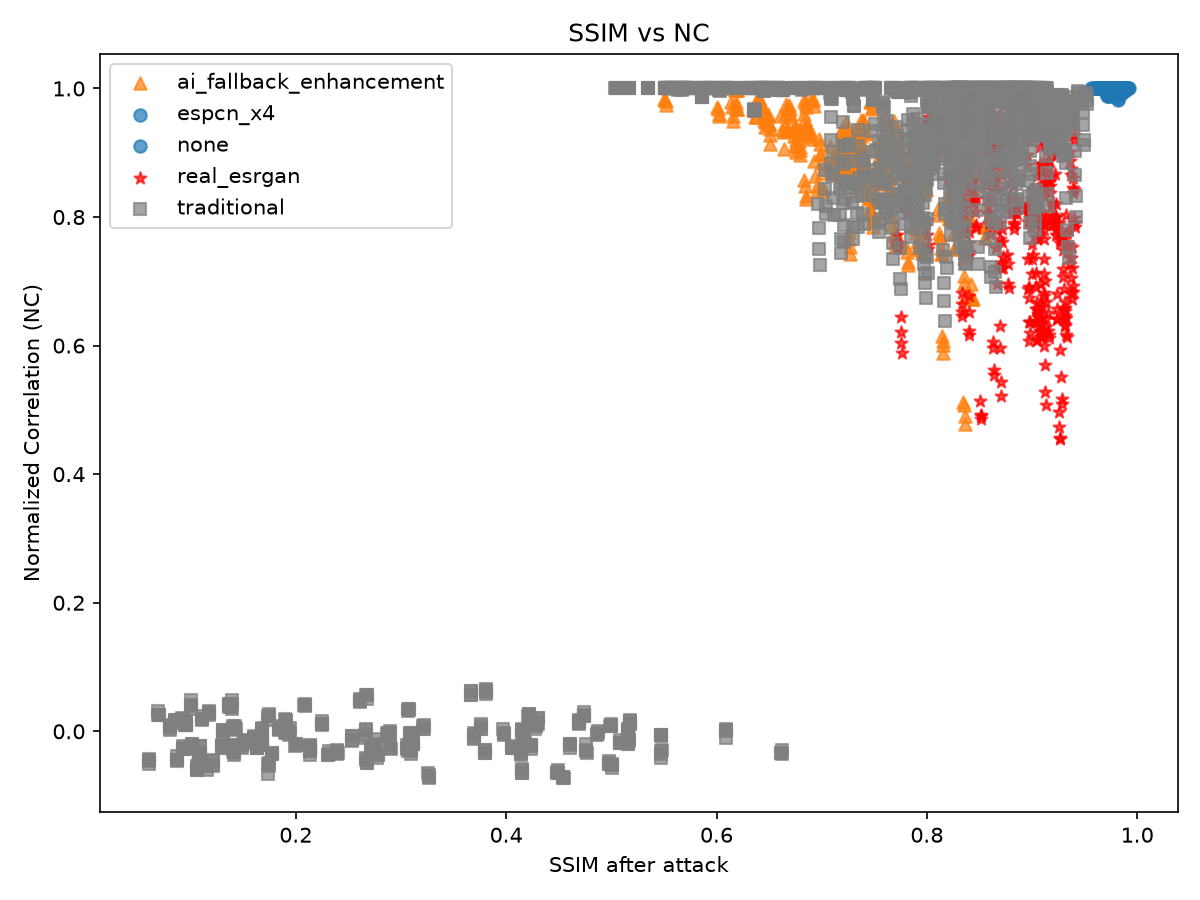
\includegraphics[width=0.88\columnwidth]{figures/ssim_vs_nc.png}
\caption{SSIM vs.\ NC per attacked image. Real-ESRGAN occupies a
high-SSIM, low-NC region unreachable by any classical attack; ESPCN
clusters near $\mathrm{NC}=1.0$ at high SSIM.}
\label{fig:asymmetry}
\end{figure}

\subsection{The Quality--Watermark Asymmetry}
Figure~\ref{fig:asymmetry} shows the central observation. Every
classical attack that reduces NC also reduces SSIM; Real-ESRGAN
decouples them, occupying a high-quality, low-detection region no
classical attack reaches. Operationally, a content owner monitoring
watermark integrity would observe degraded detection with no visible
indication the image had been modified --- a qualitatively distinct
threat.

\subsection{Embedding Strength Does Not Restore Robustness}
% SOURCE: results/metrics.csv (standard variant, attack real_esrgan,
%   100 images per alpha; src/run_experiment.py, pipeline P1).
% Regenerated 2026-07-14 per AUDIT_REPORT.md Sec. 6 (previous values were
%   from an unidentifiable earlier run; SSIM was a Kodak-only aggregate).
\begin{table}[t]
\caption{Mean NC under Real-ESRGAN by embedding strength $\alpha$,
standard pair $(4,1)/(1,4)$, averaged across 100 images.}
\label{tab:alpha_main}
\centering
\begin{tabular}{ccc}
\toprule
$\alpha$ & NC (Real-ESRGAN) & SSIM \\
\midrule
0.05 & 0.774 & 0.886 \\
0.10 & 0.783 & 0.885 \\
0.20 & 0.802 & 0.885 \\
0.30 & 0.820 & 0.884 \\
\bottomrule
\end{tabular}
\end{table}
Table~\ref{tab:alpha_main} shows NC improves only marginally
($+0.046$) as $\alpha$ increases sixfold from 0.05 to 0.30, while SSIM
remains flat. For classical
attacks, stronger embedding produces proportionally better survival;
Real-ESRGAN does not exhibit this behavior, consistent with the model
overwriting DCT coefficient relationships during reconstruction rather
than merely attenuating the embedded signal.

\section{Mechanism and Mitigation}
\label{sec:analysis}

\subsection{DCT Coefficient Damage Profiles}
\begin{figure}[t]
\centering
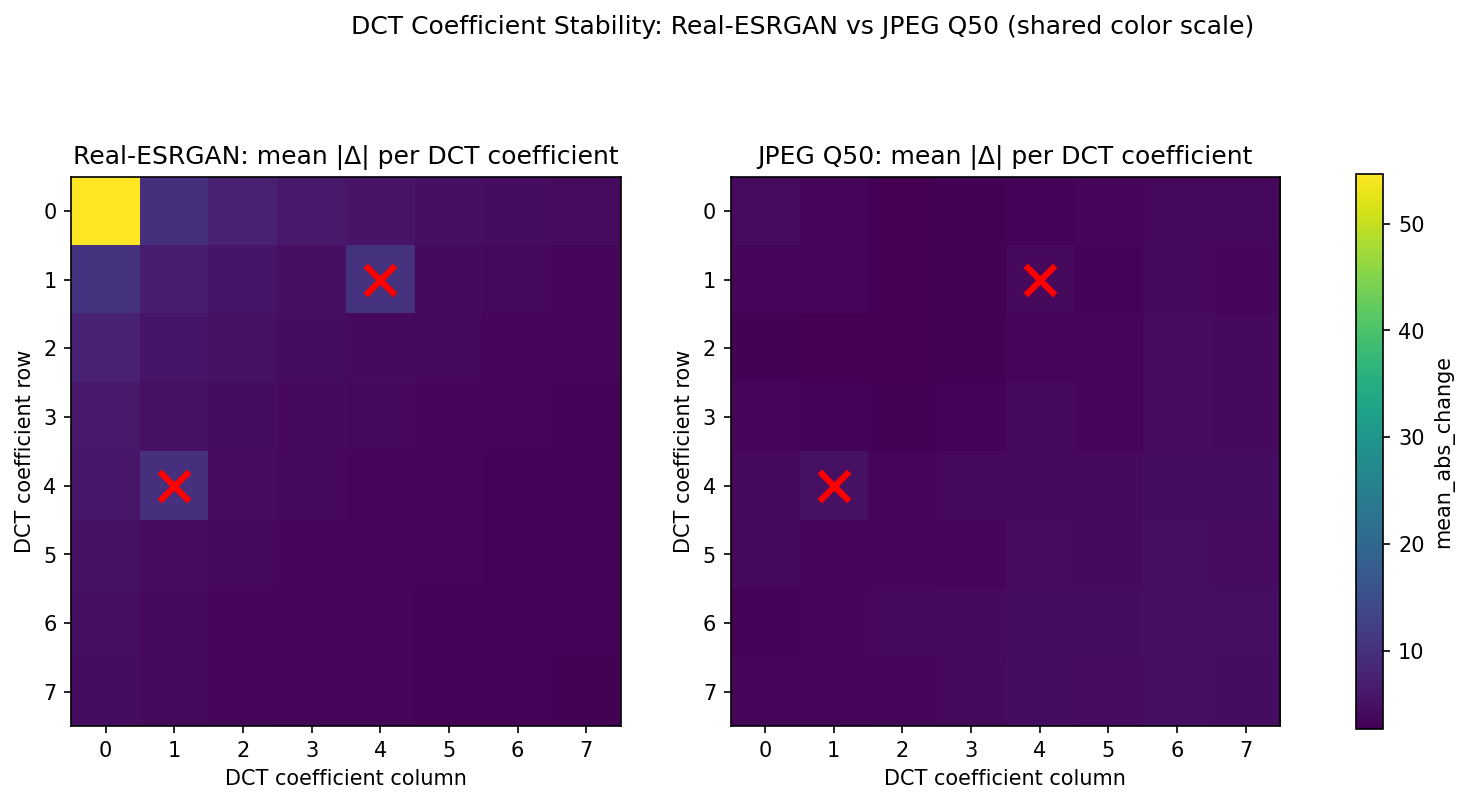
\includegraphics[width=\columnwidth]{figures/dct_stability_comparison.png}
\caption{Mean absolute DCT coefficient perturbation per position for
Real-ESRGAN (left) and JPEG-Q50 (right) across 102,400 blocks, shared
color scale. Real-ESRGAN concentrates damage in the DC coefficient;
JPEG distributes damage nearly uniformly. Baseline embedding positions
$(4,1)$ and $(1,4)$ are marked.}
\label{fig:heatmap}
\end{figure}

Figure~\ref{fig:heatmap} shows mean absolute perturbation per DCT
position. Real-ESRGAN concentrates damage almost entirely in the DC
coefficient at $(0,0)$: its mean perturbation is $5.3\times$ that of the
most-damaged non-DC position and $14\times$ the median non-DC position,
with elevated perturbation into the low- and mid-frequency region ---
consistent with the learned reconstruction re-rendering local luminance
statistics, and not attributable to resampling, since ESPCN shares that
pipeline and leaves extraction nearly perfect. JPEG-Q50 distributes damage across all
64 positions in a narrow range with mild elevation at higher frequencies,
consistent with its quantization table design.

The two profiles are strongly anti-complementary: Spearman rank
correlation between the per-position ESRGAN and JPEG damage profiles,
measured on the $\alpha$-resolved profiles of the embedding-strength
stability analysis below, is
$\rho = -0.716$ ($p < 10^{-10}$), and between the ESRGAN damage profile
and the JPEG quantization step-size vector is $\rho = -0.907$
($p < 10^{-25}$): positions most damaged by ESRGAN tend to be least
damaged by JPEG, so improving robustness to one attack by position
choice tends to hurt robustness to the other.

The classical embedding positions $(4,1)$ and $(1,4)$ sit in a
mid-frequency zone where Real-ESRGAN's perturbation is elevated relative
to the most stable high-frequency corner positions. The
coefficient-selection assumptions inherited from the compression era do
not transfer to the enhancement threat.

\subsection{Exhaustive Pair Search and Pareto Frontier}

Applying the E/J-score search of Section~\ref{sec:setup}, the Pareto
frontier --- pairs no other configuration dominates on both objectives
simultaneously --- contains 37 pairs out of 1,953. The standard baseline
pair $(4,1)/(1,4)$ lies off the frontier (E-score $= 0.028$, J-score
$= 0.877$), confirming it is not optimal under either attack in
isolation or their combination.

The anti-complementarity of the damage profiles is directly reflected at
the pair level: the ESRGAN NC and JPEG NC of individual pairs are
negatively correlated (Spearman $\rho = -0.488$, $p < 0.001$) across the
43 screened pairs, with pairs anchored near the high-frequency corner
$(7,7)$ achieving the highest ESRGAN NC and mid-frequency pairs the
highest JPEG NC (Pareto plot in the extended version). No pair improves
against both attacks simultaneously relative to the baseline.

\subsection{Three-Pair Full Validation}
\label{sec:pairs}

The three pairs of Section~\ref{sec:setup} --- standard, analytically
Pareto-optimal balanced (highest combined E+J score among the 37
Pareto-optimal pairs), and high-frequency --- are evaluated end-to-end;
Table~\ref{tab:pairs} shows results at $\alpha=0.10$.

% SOURCE: experiments/exp_F_realesrgan_pair_verification/exp_F_summary.csv
%   (nc_mean/nc_std/psnr_mean at alpha=0.10) and exp_F_tests.csv
%   (Wilcoxon BH-FDR statistics); Exp F run_exp_F.py.
% NOTE (AUDIT_REPORT.md Sec. 1/5): the balanced Real-ESRGAN arm used the
%   harsher live patch pipeline (P2); standard/HF used the disk pipeline
%   (P1). Cross-column ESRGAN comparison involving "balanced" is therefore
%   NOT like-for-like; see dagger note and text.
\begin{table}[t]
\caption{Mean NC $\pm$ standard deviation at $\alpha=0.10$, 100 images,
three pairs, four attacks. All pairwise NC differences significant after
BH--FDR correction except no-attack ($p < 10^{-12}$ or n.s.).
$^\dagger$Produced by a measurably harsher attack invocation; see the
like-for-like control in the text before comparing across columns.}
\label{tab:pairs}
\centering
\begin{tabular}{lccc}
\toprule
Attack & Standard & Balanced & HF \\
       & $(4,1)/(1,4)$ & $(2,3)/(3,2)$ & $(7,5)/(7,7)$ \\
\midrule
No attack      & $0.9997 \pm 0.000$ & $0.9997 \pm 0.000$ & $1.000 \pm 0.000$ \\
Real-ESRGAN    & $0.783 \pm 0.124$ & $0.683 \pm 0.139^\dagger$   & $0.831 \pm 0.109$ \\
JPEG-Q50       & $0.995 \pm 0.004$ & $0.998 \pm 0.001$   & $0.902 \pm 0.018$ \\
Gaussian blur  & $0.910 \pm 0.013$ & $0.933 \pm 0.011$   & $0.977 \pm 0.005$ \\
\midrule
PSNR (dB)      & $40.6$ & $40.9$ & $43.9$ \\
\bottomrule
\end{tabular}
\end{table}

\textbf{Real-ESRGAN.} The HF pair achieves NC of 0.831, 0.048 above
standard ($p < 10^{-13}$, $d = 0.89$), stable across all four embedding
strengths. The balanced pair's tabulated 0.683 must be read with care:
its Real-ESRGAN images came from a patch-based invocation of the attack,
whereas standard/HF used the whole-image invocation, and a control shows
the patch-based pipeline alone is substantially harsher ($-0.102$ NC on
the \emph{standard} pair over the same images; $n=20$, Wilcoxon
$p=10^{-4}$) --- almost exactly the apparent balanced--standard gap.
This inconsistency was identified by the decision-margin control of
Section~\ref{sec:margin}. Like-for-like, the balanced pair does
\emph{not} underperform standard (marginally better: $+0.020$, $n=20$,
$p=0.038$), with HF best under both pipelines. We therefore do not
present this comparison as final: a like-for-like rerun of the balanced
arm on all 100 images is required before camera-ready, and 0.683 is
only an upper bound on the harsher pipeline's effect. What can be
concluded already: the analytically predicted \emph{large} balanced
advantage fails to materialize under either pipeline; the next
subsection diagnoses why.

\textbf{JPEG-Q50.} The ordering reverses: Balanced ($0.998$) $>$ Standard
($0.995$) $\gg$ HF ($0.902$). The HF pair suffers a large JPEG regression
($\Delta\mathrm{NC} = -0.094$ vs.\ standard, $p < 10^{-17}$).

\textbf{Gaussian blur.} Ordering follows ESRGAN: HF ($0.977$) $>$
Balanced ($0.933$) $>$ Standard ($0.910$); all differences are large and
highly significant.

\textbf{Imperceptibility.} The balanced pair achieves higher PSNR
($+0.30$\,dB at $\alpha=0.10$), and the HF pair achieves substantially
higher PSNR ($+3.3$\,dB), eliminating below-threshold imperceptibility
failures present in the standard pair.

\textbf{Key finding.} No pair simultaneously achieves the highest NC
across all attacks, and the analytical Pareto ranking is not preserved
in magnitude end-to-end: the predicted best combined choice (balanced)
delivers only $+0.02$ like-for-like over standard under Real-ESRGAN
($n=20$ control; full rerun pending), while the HF pair --- selected by
a simpler per-position heuristic --- outperforms both. Position
selection offers attack-aware partial mitigation, but the ESRGAN/JPEG
tradeoff cannot be resolved within this scheme.

\subsection{Why the Analytical Ranking Fails: Enhancement as Endogenous
Restoration}
\label{sec:margin}

To diagnose the failure of the damage-based analytical ranking, we
measure the detector's decision statistic directly: survival is
governed by the signed margin $M = C_1 - C_2$, measured per block
before and after Real-ESRGAN for all three pairs at $\alpha = 0.10$
(307,200 blocks), together with each block's \emph{natural} margin
$M_{\mathrm{orig}}$ in the unwatermarked original. NC loss is entirely
margin sign flips (flip and bit-error rates agree to within 0.1\%);
the embedding's margin floor clamps $|M|$ near 30 for all pairs, and
pre-attack margin magnitude predicts nothing (Spearman
$\rho \approx -0.07$, n.s.). The best image-level predictor of NC is
the standard deviation of the \emph{differential} perturbation
$\sigma(\Delta C_1 - \Delta C_2)$ ($\rho = -0.887$), outperforming the
absolute per-coefficient damage used by the analytical E-score
($\rho = -0.825$); common-mode perturbation, to which the comparison
detector is blind by design, is irrelevant ($\rho = -0.22$).

The perturbation is \emph{signal-dependent}: it is anti-correlated
with the embedding-induced margin shift
($r = -0.73 / -0.60 / -0.80$ for standard/balanced/HF), removes
32\%/30\%/53\% of what the embedder inserted, and adding
$M_{\mathrm{orig}}$ to a before-only regression of the post-attack
margin raises $R^2$ from 0.71 to 0.83 (standard pair). This behavior
is inconsistent with fixed, position-dependent noise and is consistent
with learned image restoration reducing the artificial coefficient
relationships introduced by comparison-based embedding --- an
\emph{endogenous} restoration process; we characterize the model's
input--output behavior only and make no claim about its internal
computations.

Consequently, the watermark dies where it fought nature: blocks whose
natural ordering opposes the embedded bit flip at 3.4--9.5$\times$ the
rate of agreeing blocks, and 77--91\% of all flips occur in that
$\approx$50\% of blocks. This suggests why the HF pair survives best
despite the largest restoration fraction (53\%): its natural margins
are tiny (mean $|M_{\mathrm{orig}}| = 10.1$ vs.\ $\approx 31$ for the
other pairs), consistent with a restoration process having little to
restore against the embedded ordering. The governing quantity for
position selection is thus the \emph{differential perturbation of the
embedded coefficient pair}, not per-position exogenous damage. Full
derivations and additional analyses appear in the extended version.

\subsection{Generalization Across Super-Resolution Architectures}
\label{sec:generalization}

% SOURCE: experiments/exp_I_sr_model_generalization/
%   {mechanism_summary_exp_I.csv, restoration_regression_exp_I.csv}
%   (Exp I analyze_exp_I.py). Real-ESRGAN row = frozen Exp H standard-pair
%   rows (block_margins.csv, pipeline P1), not recomputed.
\begin{table}[t]
\caption{Margin-analysis mechanism quantities per SR model (standard
pair, $\alpha=0.10$, 102,400 blocks per model). $k$ = fraction of the
embedded coefficient differential removed; $r_{\mathrm{undo}}$ =
correlation between differential perturbation and embedded shift.}
\label{tab:mechanism}
\centering
\begin{tabular}{lcccc}
\toprule
Model & Flip rate & $\sigma(\Delta C_1{-}\Delta C_2)$ & $k$ & $r_{\mathrm{undo}}$ \\
\midrule
ESPCN $4\times$       & 0.02\% & 1.9  & 0.5\%  & $-0.14$ \\
FSRCNN $4\times$      & 0.01\% & 1.8  & 0.2\%  & $-0.05$ \\
EDSR $4\times$        & 0.00\% & 0.6  & 0.2\%  & $-0.20$ \\
LapSRN $4\times$      & 0.02\% & 3.7  & 4.7\%  & $-0.69$ \\
Real-ESRGAN $4\times$ & 10.9\% & 24.2 & 32.3\% & $-0.73$ \\
\bottomrule
\end{tabular}
\end{table}

Is this pressure unique to Real-ESRGAN? Repeating the margin analysis
at $\alpha = 0.10$ (standard pair) for the four PSNR-oriented models
(Table~\ref{tab:mechanism}) shows differential perturbation an order of
magnitude below the $\approx$30-unit enforced margin ($\sigma =
0.6$--$3.7$ vs.\ 24.2), so essentially no block crosses the decision
boundary. EDSR (43\,M parameters) is the most transparent model tested:
training objective, not capacity, separates harmless from damaging
models. LapSRN is the instructive intermediate case: its perturbation
\emph{direction} carries nearly the same restoration signature as
Real-ESRGAN ($r_{\mathrm{undo}} = -0.69$ vs.\ $-0.73$) at $7\times$
weaker strength ($k = 4.7\%$ vs.\ 32.3\%), and the few flips these
models cause occur exclusively in blocks whose natural ordering opposes
the embedded bit --- the same signature, in miniature. A perturbation
component directed against the embedded relationship is thus present
across the learned SR architectures we test, but on current evidence
only the GAN-trained restoration model is strong enough to cross the
decision boundary: the practical threat is architecture-dependent, not
a property of ``AI enhancement'' as a category.

\subsection{Stability of the Anti-Complementarity Across Embedding Strengths}

Measuring the per-position ESRGAN and JPEG damage profiles at all four
$\alpha$ values (standard pair), the anti-complementarity is essentially
constant: $\rho$ ranges from $-0.716$ at $\alpha=0.05$ to $-0.706$ at
$\alpha=0.30$, a total range of 0.010 over a $6\times$ span of embedding
strength, and the Jaccard similarity of the top-10 most-damaged
positions is 1.0 for all cross-$\alpha$ comparisons, for both attacks
independently. The anti-complementarity is thus a structural property of
the two attack types, not of the embedding strength; Real-ESRGAN damage
isotropy is similarly stable ($r \approx 0.989$) across all tested
$\alpha$. The margin analysis of Section~\ref{sec:margin} gives this a
mechanistic reading: JPEG's damage follows its fixed quantization table
while Real-ESRGAN's follows the embedded signal itself --- consistent
with mechanistically different kinds of noise, which would explain why
no static position choice escapes the trade-off.

% SOURCE: results/symmetry_summary.csv (src/frequency_sweep.py screening
%   runs, pipeline P1).
Separately, symmetric coefficient pairs achieve mean Real-ESRGAN NC of
0.821 versus 0.689 for asymmetric pairs (43-pair screening set,
$\alpha=0.1$, 20-image subset), disconfirming coordinate symmetry as
the cause of Real-ESRGAN vulnerability.

\subsection{Subband Selection Does Not Help}
% SOURCE: results/comparison_metrics.csv (src/run_comparison.py,
%   alpha=0.1, 100 images, pipeline P1).
A supplementary DWT-SVD-HH scheme at matched imperceptibility (47.7
vs.\ 48.0\,dB, $\alpha=0.1$) achieves NC of only 0.18/0.18/0.29 (blur,
JPEG-Q50, Real-ESRGAN) where DWT-DCT-LL survives at 0.93/0.98/0.74:
high-frequency subbands are not a viable escape.

\subsection{Limitations}
Our evaluation covers five learned super-resolution architectures;
within this set the destructive behavior is confined to the GAN-trained
restoration model; diffusion-based enhancers and other GAN restorers
remain untested. The margin analysis is reported at $\alpha=0.10$ only,
and the balanced-pair like-for-like control (Section~\ref{sec:pairs})
remains $n=20$ pending the camera-ready rerun.
All headline results are for one classical scheme (DWT-DCT with
ordering-based bit encoding); generalization to other classical schemes
remains to be established.
The Pareto analysis uses proxy scores rather than end-to-end NC;
Section~\ref{sec:margin} suggests why such proxies mispredict for
generative attacks (they model a signal-dependent attack as exogenous
noise), and the $|M_{\mathrm{orig}}|$ selection rule has not yet been
validated prospectively on new pairs.

\section{Conclusion}
\label{sec:conclusion}

AI-based image enhancement can violate the quality--attack tradeoff
underlying classical watermark robustness evaluation: Real-ESRGAN
degrades DWT-DCT
watermark recovery to NC $= 0.795$ at the highest perceptual quality
(SSIM 0.885) of any watermark-degrading attack tested, while ESPCN,
FSRCNN, EDSR, and LapSRN --- sharing the identical resampling pipeline ---
leave watermarks intact. The decision-margin analysis shows that what
governs survival is the \emph{differential perturbation of the embedded
coefficient pair}, not absolute coefficient stability: the perturbation
selectively removes the embedded coefficient differential --- consistent
with learned restoration reducing the artificial relationships
introduced by comparison-based embedding --- so that failures
concentrate where the natural ordering opposes the embedded bit.
PSNR-oriented models show the same direction at an order of magnitude
lower strength: on current evidence the threat is
architecture-dependent, not a property of learned enhancement. No coefficient pair simultaneously maximizes Real-ESRGAN and
JPEG robustness, and this anti-complementarity is stable across all
tested embedding strengths, consistent with its exogenous-vs-endogenous
origin rather than tuning.

Content owners relying on DWT-DCT watermarking should be aware that
consumer enhancement tools built on GAN-trained restoration can
silently degrade watermark integrity, while common PSNR-oriented
super-resolvers do not. Attack-aware coefficient selection offers
partial mitigation: the high-frequency pair $(7,5)/(7,7)$ improves
Real-ESRGAN NC from 0.795 to 0.831 and eliminates imperceptibility
failures at the cost of JPEG NC (0.996 to 0.902); the margin analysis
suggests an explanation --- near-zero natural margins leave a
restoration-type attack little to restore --- yielding a candidate
selection rule (minimize natural $|M_{\mathrm{orig}}|$) in place of
per-position damage heuristics. Future work should validate this rule prospectively, extend to
diffusion-based enhancers and additional GAN restorers, and investigate
content-adaptive strategies against both attack types.

\section*{Acknowledgment}
The author used Claude (Anthropic) as an AI coding assistant for
pipeline implementation; all experimental design, analysis, and
writing are the author's own.

\bibliographystyle{IEEEtran}
\bibliography{references_revised}

\end{document}
